
\documentclass{standalone}

\usepackage{tikz}
\usepackage{circuitikz}

\begin{document}

%%%%\begin{figure}[!ht]
%%%%\centering
%%%\begin{tikzpicture}[line width=1pt]
%%%\draw (0.0,0.0) to [short, -o] (0.0,1.0) node[left] {$-$};
%%%\draw (0.0,1.0) to [open, l=$U_1$,inner sep=10pt] (0.0,1.5);
%%%\draw (0.0,1.5) node[left] {$+$} to [short, o-] (0.0,2.5);
%%%
%%%\draw (0.0,2.5) to [short, -o] (1.0,2.5) node[above] {$-$};
%%%\draw (1.0,2.5) to [open, n=uII] (1.5,2.5); \node[above=4pt] at (uII.n) {$U_2$};
%%%\draw (1.5,2.5) node[above] {$+$} to [short, o-] (2.5,2.5);
%%%
%%%\draw (2.5,2.5) to [short, -o] (2.5,1.5) node[right] {$-$};
%%%\draw (2.5,1.5) to [open, l=$U_3$, inner sep=10pt] (2.5,1.0);
%%%\draw (2.5,1.0) node[right] {$+$} to [short, o-] (2.5,0.0);
%%%
%%%\draw (2.5,0.0) to [short, -o] (1.5,0.0) node[below] {$-$};
%%%\draw (1.5,0.0) to [open, n=uIV] (1.0,0.0); \node[below=4pt] at (uIV.n) {$U_4$};
%%%\draw (1.0,0.0) node[below] {$+$} to [short, o-] (0.0,0.0);
%%%\end{tikzpicture}
%%%%\caption{De spanningswet van Kirchoff: alle spanningen in een kring zijn opgeteld 0.}
%%%%\label{fig:spanningswetkirchoff}
%%%%\end{figure}

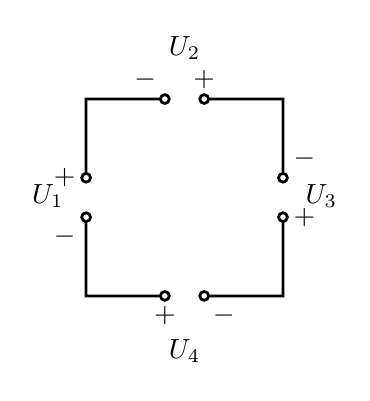
\begin{tikzpicture}[line width=1pt]

\draw (0.0,0.0)  node[left] {$+$} to [short, o-] ++(0.0,1.0) to [short, -o]  node[above] {$-$} ++(1.0,0.0)
      to [open,l=$U_2$,above] ++(0.5,0.0) node[above] {$+$} to [short, o-] ++(1.0,0.0) to [short, -o] node[right] {$-$} ++(0.0,-1.0)
      to [open,l=$U_3$,inner sep=8pt] ++(0.0,-0.5) node[right] {$+$} to [short, o-] ++(0.0,-1.0) to [short, -o] node[below] {$-$} ++(-1.0,0.0)
      to [open,l=$U_4$,above] ++(-0.5,0.0) node[below] {$+$} to [short, o-] ++(-1.0,0.0) to [short, -o] node[left] {$-$} ++(0.0,1.0)
      to [open,l=$U_1$,inner sep=8pt] ++(0.0,0.5)
;
\end{tikzpicture}




\end{document}
